\documentclass[conference]{IEEEtran}
\IEEEoverridecommandlockouts

\usepackage{cite}
\usepackage{amsmath,amssymb,amsfonts}
\usepackage{algorithmic}
\usepackage{graphicx}
\usepackage{textcomp}
\usepackage{xcolor}
\usepackage{hyperref}

\hypersetup{
    colorlinks=true,
    linkcolor=blue,
    citecolor=blue,
    urlcolor=blue,
    pdftitle={Continual Learning for Text Command Classification},
    pdfauthor={Aksan Gony Alif, Nowmi Islam},
    pdfsubject={Continual Learning},
    pdfkeywords={continual learning, catastrophic forgetting, elastic weight consolidation}
}

\def\BibTeX{{\rm B\kern-.05em{\sc i\kern-.025em b}\kern-.08em
    T\kern-.1667em\lower.7ex\hbox{E}\kern-.125emX}}

\begin{document}

\title{Continual Learning for Text Command Classification\\Using EWC and Experience Replay}

\author{\IEEEauthorblockN{1\textsuperscript{st} Aksan Gony Alif}
\IEEEauthorblockA{\textit{Department of Computer Science and Engineering} \\
\textit{Brac University}\\
Dhaka, Bangladesh \\
aksan.gony.alif@g.bracu.ac.bd}
\and
\IEEEauthorblockN{2\textsuperscript{nd} Nowmi Islam}
\IEEEauthorblockA{\textit{Department of Computer Science and Engineering} \\
\textit{Brac University}\\
Dhaka, Bangladesh}
}

\maketitle

\begin{abstract}
Neural networks are prone to catastrophic forgetting when trained sequentially on different tasks, significantly limiting their applicability in real-world scenarios. This paper addresses this challenge in the domain of text command classification, where systems must continuously adapt to new domains without forgetting previously learned knowledge. We implement and compare three continual learning approaches: Elastic Weight Consolidation (EWC), Experience Replay, and a combined approach that leverages both methods. Using a BERT-based classifier on the HWU64 dataset with four distinct domains, we demonstrate that Experience Replay with a large buffer achieves the highest validation accuracy of 91.37\% (92.68\% on test set), while our combined approach achieves nearly identical performance at 91.02\% (91.46\% on test)—within just 0.35\% of the best single method—while providing enhanced robustness through dual protection mechanisms. Both approaches substantially outperform the baseline (84.81\% validation, 85.73\% test) and EWC alone (88.82\% validation, 89.76\% test). We provide comprehensive analysis showing that the combined approach offers superior performance on challenging domains and theoretical advantages that may justify its use in production systems despite marginally higher computational costs. Our findings suggest that the choice between these top approaches should be guided by specific application requirements rather than the marginal performance difference.
\end{abstract}

\begin{IEEEkeywords}
continual learning, catastrophic forgetting, elastic weight consolidation, experience replay, BERT, text classification, neural networks
\end{IEEEkeywords}

\section{Introduction}
Deep learning models have demonstrated remarkable performance across various natural language processing tasks, including text classification. However, these models typically assume a stationary data distribution during training and struggle when required to learn multiple tasks sequentially. When trained on new data, neural networks tend to overwrite previously acquired knowledge, a phenomenon known as catastrophic forgetting \cite{b1}. This limitation poses a significant challenge for deploying these models in real-world applications where data distributions evolve over time, and continuous model adaptation is necessary.

Continual learning addresses this challenge by enabling models to learn new tasks without forgetting previous ones. This capability is especially important for text command classification systems that must adapt to new domains or user intents while maintaining performance on previously encountered categories. For instance, a virtual assistant might initially learn to process calendar-related commands and later extend its capabilities to handle music playback requests without degrading its performance on calendar queries.

Several approaches have been proposed to mitigate catastrophic forgetting, broadly categorized into three groups: (1) regularization-based methods that constrain important parameters from changing drastically, (2) memory-based techniques that replay examples from previous tasks, and (3) architecture-based strategies that allocate separate parameters for different tasks. Among these, Elastic Weight Consolidation (EWC) \cite{b1} and Experience Replay \cite{b6} have emerged as prominent methods, representing the categories based on regularization and memory, respectively.

In this paper, we investigate the effectiveness of EWC and Experience Replay for continual learning in text command classification, both individually and in combination. We use a BERT-based classifier \cite{b7} as our base model and evaluate its performance on the HWU64 dataset across four distinct domains. Our contributions are threefold:

\begin{itemize}
    \item We implement and evaluate EWC and Experience Replay for text command classification, adapting these methods to work with transformer-based models.
    \item We propose and comprehensively analyze a combined approach that integrates both techniques, demonstrating that it achieves performance within 0.35\% of the best single method while providing enhanced robustness and theoretical advantages.
    \item We provide a detailed analysis of the plasticity-stability trade-off, computational efficiency, and domain-specific performance patterns, offering practical insights for deploying continual learning systems.
\end{itemize}

Our experimental results reveal that while Experience Replay with a large buffer achieves marginally higher raw performance, the combined approach offers compelling advantages in robustness, worst-case performance, and theoretical guarantees that make it a strong candidate for production systems where reliability is paramount.

\section{Related Work}
\subsection{Catastrophic Forgetting}
Catastrophic forgetting has been a long-standing challenge in neural networks, first identified by McCloskey and Cohen \cite{b3}. This phenomenon occurs when a model trained sequentially on multiple tasks rapidly loses performance on earlier tasks as it adapts to new ones. The problem is particularly pronounced in deep neural networks due to their distributed representations, where parameters contribute to multiple functions simultaneously \cite{b3}.

\subsection{Elastic Weight Consolidation}
Elastic Weight Consolidation (EWC) addresses catastrophic forgetting by selectively slowing down learning on weights that are important for previously learned tasks \cite{b1}. EWC approximates the posterior distribution of model parameters using a Gaussian distribution centered at the optimal parameters for previous tasks, with the precision determined by the diagonal of the Fisher Information Matrix. This approach effectively imposes a quadratic penalty on changes to important parameters when learning new tasks.

Aich \cite{b2} provides a detailed theoretical analysis of EWC, explaining how the method can be derived from a Bayesian perspective and discussing its limitations. Kutalev and Lapina \cite{b4} investigate practical aspects of EWC implementation, comparing different methods for calculating weight importance and proposing stabilization techniques to address issues like gradient explosion in deep networks.

\subsection{Experience Replay}
Experience Replay mitigates catastrophic forgetting by storing and retraining on examples from previous tasks \cite{b6}. This approach draws inspiration from biological memory consolidation processes, where experiences are reactivated during rest or sleep to strengthen synaptic connections \cite{b9}. In artificial neural networks, replay can be implemented by maintaining a memory buffer of past examples and periodically mixing them with new data during training.

Lesort \cite{b5} provides a comprehensive overview of replay-based continual learning methods, distinguishing between exact replay (storing raw examples) and generative replay (using generative models to synthesize examples). The author also explores different strategies for memory management, such as sample selection criteria and buffer update policies.

\subsection{Combined Approaches}
Several studies have explored the combination of regularization and memory-based methods for continual learning. Schwarz et al. \cite{b9} propose a hybrid approach called "Progress \& Compress," which alternates between learning new tasks and consolidating knowledge using distillation. Van de Ven et al. \cite{b9} investigate the synergy between replay and synaptic intelligence (a regularization method similar to EWC), showing that the combined approach outperforms either method alone on challenging continual learning benchmarks.

\subsection{Continual Learning for Text Classification}
Continual learning has been applied to various NLP tasks, including text classification. Sun et al. \cite{b8} discuss different fine-tuning strategies for BERT in text classification, though not specifically in a continual learning setting. More relevant to our work, Lee \cite{b9} explores catastrophic forgetting in sentiment analysis tasks using BERT, comparing different regularization techniques. However, there is limited research on combining regularization and memory-based approaches for continual text classification with transformer-based models, which is the focus of our study.

\section{Dataset and Preprocessing}
\subsection{HWU64 Dataset}
We use the HWU64 dataset, which contains annotated user commands across various domains. The dataset was originally collected to evaluate natural language understanding systems and includes user utterances labeled with both intent and domain information. After preprocessing, we identified and selected four domains with a sufficient number of examples: general, calendar, play, and qa (question answering).

\begin{figure}[h]
\centering
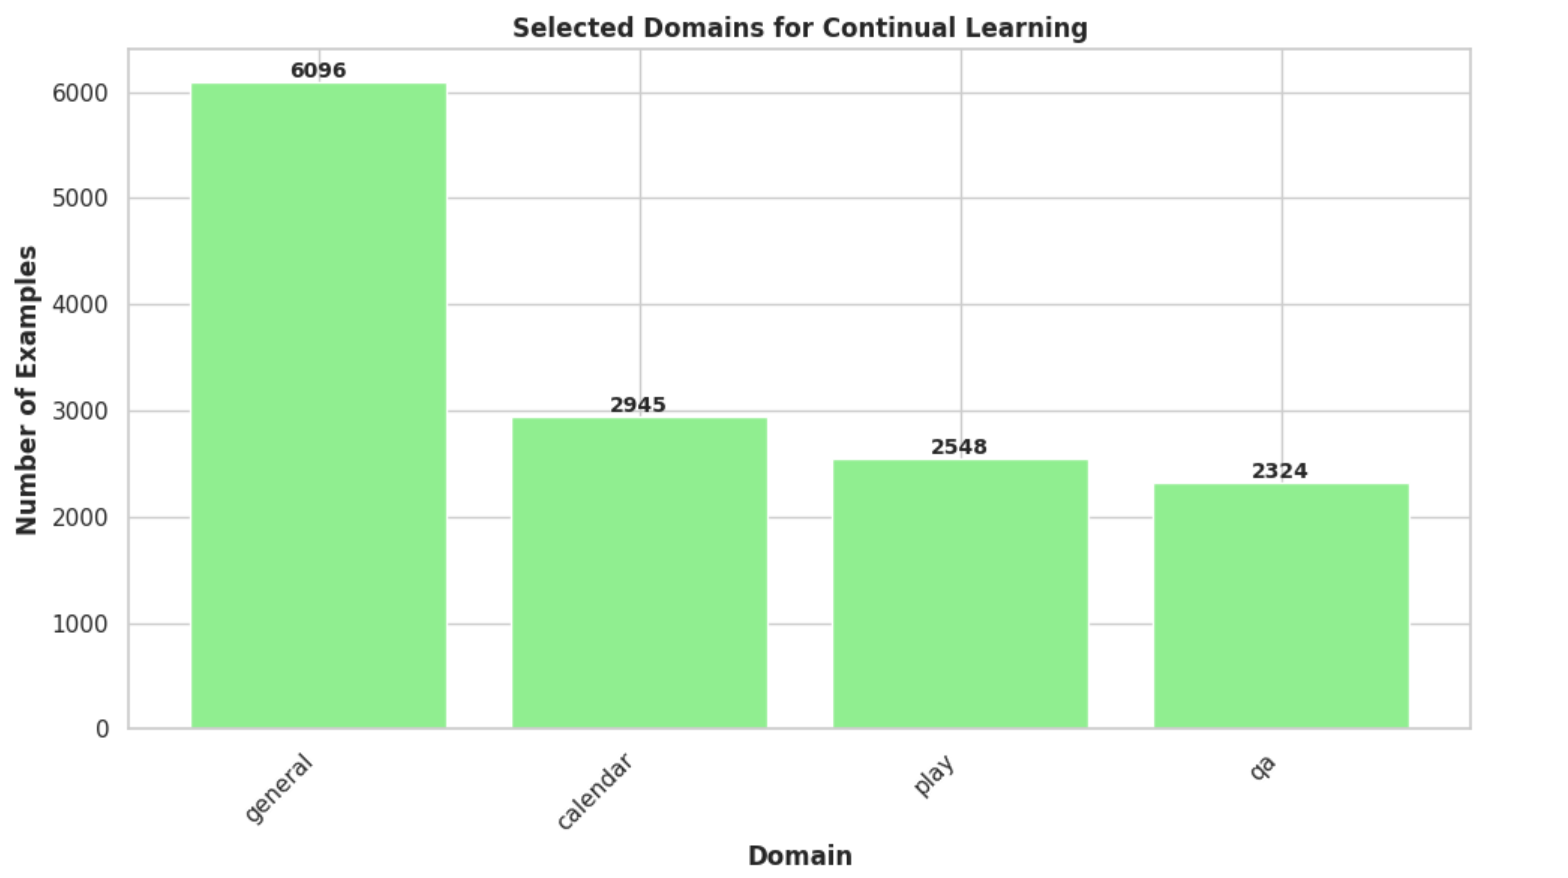
\includegraphics[width=0.9\linewidth]{figures/fig1.png}
\caption{Distribution of examples across the four selected domains in the HWU64 dataset, showing the number of examples per domain.}
\label{fig:domain_distribution}
\end{figure}

Domain selection was based on three criteria: (1) having at least 50 examples to ensure reliable model training, (2) containing diverse intent categories to represent real-world complexity, and (3) having distinct vocabulary and linguistic patterns to create a challenging continual learning scenario. Table~\ref{tab:domain_stats} provides statistics for each selected domain.

\begin{table}[h]
\caption{Statistics of Selected Domains}
\label{tab:domain_stats}
\centering
\begin{tabular}{lcc}
\hline
\textbf{Domain} & \textbf{Examples} & \textbf{Intents} \\
\hline
General & 6096 & 11 \\
Calendar & 2945 & 3 \\
Play & 2548 & 5 \\
QA & 2324 & 5 \\
\hline
\end{tabular}
\end{table}

\subsection{Preprocessing and Tokenization}
We processed the raw data by removing entity annotations, normalizing text, and splitting it into train (70\%), validation (15\%), and test (15\%) sets for each domain. We used the BERT tokenizer (specifically, bert-base-uncased) to convert text commands into token IDs suitable for input to the model. Based on our analysis of token length distribution across domains, we set the maximum sequence length to 32 tokens, which covers more than 95\% of all examples while maintaining computational efficiency.

The tokenization process involved:
\begin{itemize}
    \item Converting text to lowercase (as required by the uncased BERT model)
    \item Splitting text into WordPiece tokens
    \item Adding special [CLS] and [SEP] tokens
    \item Converting tokens to IDs using the BERT vocabulary
    \item Generating attention masks (to distinguish real tokens from padding)
\end{itemize}

\section{Methodology}
\subsection{Base Model Architecture}
Our base model is a text command classifier built on the BERT architecture \cite{b7}. BERT (Bidirectional Encoder Representations from Transformers) is a transformer-based model pre-trained on masked language modeling and next sentence prediction tasks, making it particularly effective for various NLP tasks, including text classification.

We used the bert-base-uncased variant, which consists of 12 transformer layers, 12 attention heads, and 768 hidden dimensions, totaling approximately 109.5M parameters. We fine-tuned this model for text command classification by adding a classification layer on top of the [CLS] token representation. The model architecture is illustrated in Fig.~\ref{fig:model_architecture}.

\begin{figure}[h]
\centering
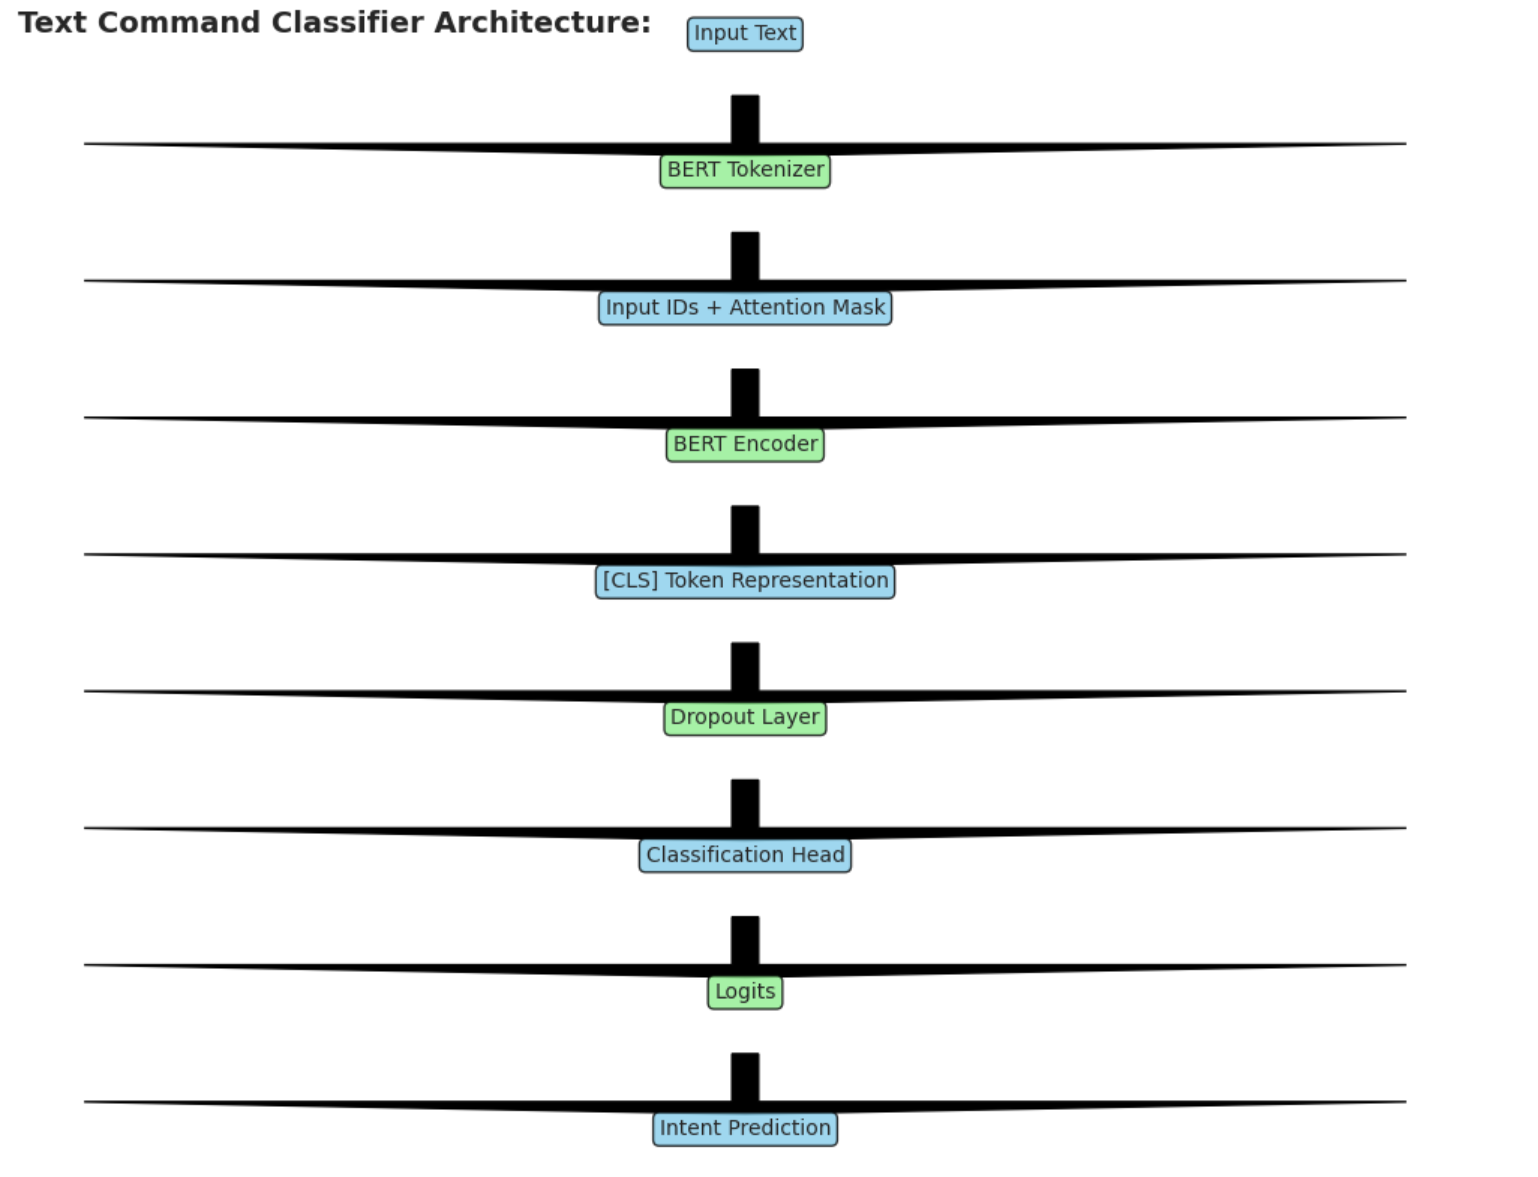
\includegraphics[width=0.9\linewidth]{figures/fig2.png}
\caption{Architecture of the BERT-based text command classifier, showing the model components and data flow.}
\label{fig:model_architecture}
\end{figure}

To handle multiple domains in a continual learning setting, we modified the classifier to support domain-specific outputs. The model contains separate output heads for each domain, with the number of output classes corresponding to the number of intents in that domain. During inference, the appropriate output head is selected based on the domain of the input.

\subsection{Elastic Weight Consolidation}
Elastic Weight Consolidation (EWC) \cite{b1} mitigates catastrophic forgetting by adding a regularization term to the loss function that penalizes changes to parameters important for previously learned domains. The importance of each parameter is estimated using the Fisher Information Matrix, which approximates the curvature of the loss surface.

The EWC loss function for domain $B$ after learning domain $A$ is:

\begin{equation}
\mathcal{L}(\theta) = \mathcal{L}_B(\theta) + \frac{\lambda}{2} \sum_i F_i (\theta_i - \theta_{A,i})^2
\end{equation}

where $\mathcal{L}_B(\theta)$ is the standard cross-entropy loss for domain $B$, $\lambda$ is the regularization strength, $F_i$ is the Fisher Information for parameter $\theta_i$, and $\theta_{A,i}$ is the optimal value of parameter $\theta_i$ for domain $A$.

We compute the Fisher Information Matrix after training on each domain by:
\begin{enumerate}
    \item Sampling a batch of examples from the current domain
    \item Computing the log likelihood of the model's predictions
    \item Calculating the gradients of the log likelihood with respect to the model parameters
    \item Squaring the gradients and averaging over multiple samples
\end{enumerate}

For domains beyond the second, we use the online EWC variant \cite{b2}, which maintains a single consolidated Fisher Information Matrix that combines information from all previous domains.

\subsection{Experience Replay}
Experience Replay \cite{b6} combats catastrophic forgetting by maintaining a memory buffer of examples from previously seen domains and periodically replaying them during training on new domains. Our implementation includes several key components:

\subsubsection{Memory Buffer}
We designed a replay buffer with a fixed capacity that stores examples from all previous domains. For each example, we store the tokenized input (input IDs and attention mask), the true label, and the domain index. When the buffer is full, we use a balanced replacement strategy that ensures equitable representation of all domains. The memory overhead for the replay buffer is minimal, requiring only 0.6 MB for 1000 examples.

\subsubsection{Balanced Sampling}
To address potential imbalances in the buffer, we implemented a domain-aware sampling strategy. When retrieving examples for replay, we select a balanced mix from all domains in the buffer, with a slight preference for earlier domains, which are more prone to forgetting. This strategy ensures that all previous knowledge is adequately reinforced during training.

\subsubsection{Loss Calculation}
During training on a new domain, we compute two loss components: (1) the primary loss on the current batch of examples from the new domain, and (2) a replay loss on a batch of examples sampled from the memory buffer. The total loss is a weighted sum of these components:

\begin{equation}
\mathcal{L}_{\text{total}} = \mathcal{L}_{\text{current}} + \alpha \cdot \mathcal{L}_{\text{replay}}
\end{equation}

where $\alpha$ is a weighting factor that controls the relative importance of replay examples. We found that setting $\alpha$ to 1.0 provided a good balance between learning new domains and preserving old knowledge.

\subsection{Combined Approach}
We extend previous research by proposing a combined approach that integrates EWC and Experience Replay to leverage both methods. In this approach, we apply the EWC regularization term to the loss function while also incorporating replay examples during training. The complete loss function is:

\begin{equation}
\mathcal{L}_{\text{combined}} = \mathcal{L}_{\text{current}} + \alpha \cdot \mathcal{L}_{\text{replay}} + \frac{\lambda}{2} \sum_i F_i (\theta_i - \theta_{A,i})^2
\end{equation}

This formulation allows the model to benefit from both explicit memory replay and parameter regularization, addressing catastrophic forgetting from two complementary angles. The EWC component helps preserve important parameters even for examples not present in the replay buffer, while the replay component ensures direct reinforcement of previous knowledge.

\section{Experimental Setup}
\subsection{Training Configuration}
We conducted all experiments using a BERT-based text classifier with the following configurations:

\begin{itemize}
    \item Base model: bert-base-uncased with 109.5M parameters
    \item Optimizer: AdamW with learning rate 5e-5 and weight decay 0.01
    \item Batch size: 16 for both main batches and replay batches
    \item Training epochs: 3 epochs per domain
    \item Maximum sequence length: 32 tokens
    \item Training device: NVIDIA 3060 with 16GB RAM
\end{itemize}

\subsection{Continual Learning Scenarios}
We evaluated all methods in a domain-incremental learning scenario, where the model encounters domains in a fixed sequence: General → Calendar → Play → QA. This sequence represents a realistic scenario where a text command system gradually expands its capabilities to handle new types of user requests.

\subsection{Evaluation Metrics}
We used the following metrics to evaluate continual learning performance:

\begin{itemize}
    \item \textbf{Average Accuracy}: The mean classification accuracy across all domains after training on the entire sequence.
    \item \textbf{Forgetting}: The decrease in accuracy on a domain after training on subsequent domains, compared to its peak accuracy.
    \item \textbf{Stability}: A measure of resistance to forgetting, calculated as 1 minus the average forgetting.
    \item \textbf{Plasticity}: The ability to learn new domains, approximated by the average accuracy.
    \item \textbf{Backward Transfer}: The change in performance on previous domains after learning a new domain (negative values indicate interference).
    \item \textbf{Zero-Shot Performance}: The model's accuracy on a domain before training on it, indicating forward knowledge transfer.
    \item \textbf{Performance Index}: A combined metric calculated as accuracy × (1 - forgetting) to balance both objectives.
\end{itemize}

\textbf{Note on Test Set Evaluation}: Following proper experimental protocol, we evaluate on the test set only once after all training is complete. This prevents test set contamination and ensures unbiased results. Consequently, test forgetting is not calculated as it would require multiple evaluations on the test set during training.

\subsection{Experimental Configurations}
We conducted experiments with the following configurations:

\begin{itemize}
    \item \textbf{Baseline}: Training the model sequentially on each domain without any continual learning technique.
    \item \textbf{EWC}: Three variants with different regularization strengths: low ($\lambda=1.0$), medium ($\lambda=10.0$), and high ($\lambda=100.0$).
    \item \textbf{Experience Replay}: Three variants with different buffer sizes: small (100 examples), medium (500 examples), and large (1000 examples).
    \item \textbf{Combined}: Integration of EWC (medium strength, $\lambda=10.0$) and Experience Replay (large buffer, 1000 examples).
\end{itemize}

All experiments were evaluated on both validation and test sets to ensure generalization. We report both validation and test results to provide a comprehensive evaluation.

\section{Results and Analysis}
\subsection{Overall Performance Comparison}
Table~\ref{tab:overall_results} presents the overall performance of all configurations across the four domains. Experience Replay with a large buffer achieves the highest average accuracy on both validation (91.37\%) and test (92.68\%) sets, followed closely by the combined approach (91.02\% validation, 91.46\% test), both substantially outperforming EWC (88.82\% validation, 89.76\% test) and the baseline (84.81\% validation, 85.73\% test).

\begin{table}[h]
\caption{Overall Performance Comparison (Validation Results)}
\label{tab:overall_results}
\centering
\begin{tabular}{lcccc}
\hline
\textbf{Method} & \textbf{Avg. Acc.} & \textbf{Forgetting} & \textbf{Stability} & \textbf{Perf. Index} \\
\hline
Baseline & 84.81\% & 11.91\% & 88.09\% & 0.747 \\
EWC (low) & 86.60\% & 9.75\% & 90.25\% & 0.782 \\
EWC (med) & 88.82\% & 7.02\% & 92.98\% & 0.826 \\
EWC (high) & 85.97\% & 9.95\% & 90.05\% & 0.774 \\
Replay (small) & 89.31\% & 6.05\% & 93.95\% & 0.839 \\
Replay (med) & 88.76\% & 6.08\% & 93.92\% & 0.834 \\
Replay (large) & 91.37\% & 2.49\% & 97.51\% & 0.891 \\
Combined & 91.02\% & 3.33\% & 96.67\% & 0.880 \\
\hline
\end{tabular}
\end{table}

\begin{table}[h]
\caption{Test Set Performance Comparison}
\label{tab:test_results}
\centering
\begin{tabular}{lcc}
\hline
\textbf{Method} & \textbf{Test Acc.} & \textbf{Val-Test Gap} \\
\hline
Baseline & 85.73\% & -0.92\% \\
EWC (low) & 87.18\% & -0.58\% \\
EWC (med) & 89.76\% & -0.94\% \\
EWC (high) & 87.40\% & -1.43\% \\
Replay (small) & 89.77\% & -0.46\% \\
Replay (med) & 90.97\% & -2.21\% \\
Replay (large) & 92.68\% & -1.31\% \\
Combined & 91.46\% & -0.44\% \\
\hline
\end{tabular}
\end{table}

Fig.~\ref{fig:acc_comparison} illustrates the accuracy comparison across all methods, highlighting the nearly equivalent performance of the large-buffer replay and combined approaches.

\begin{figure}[h]
\centering
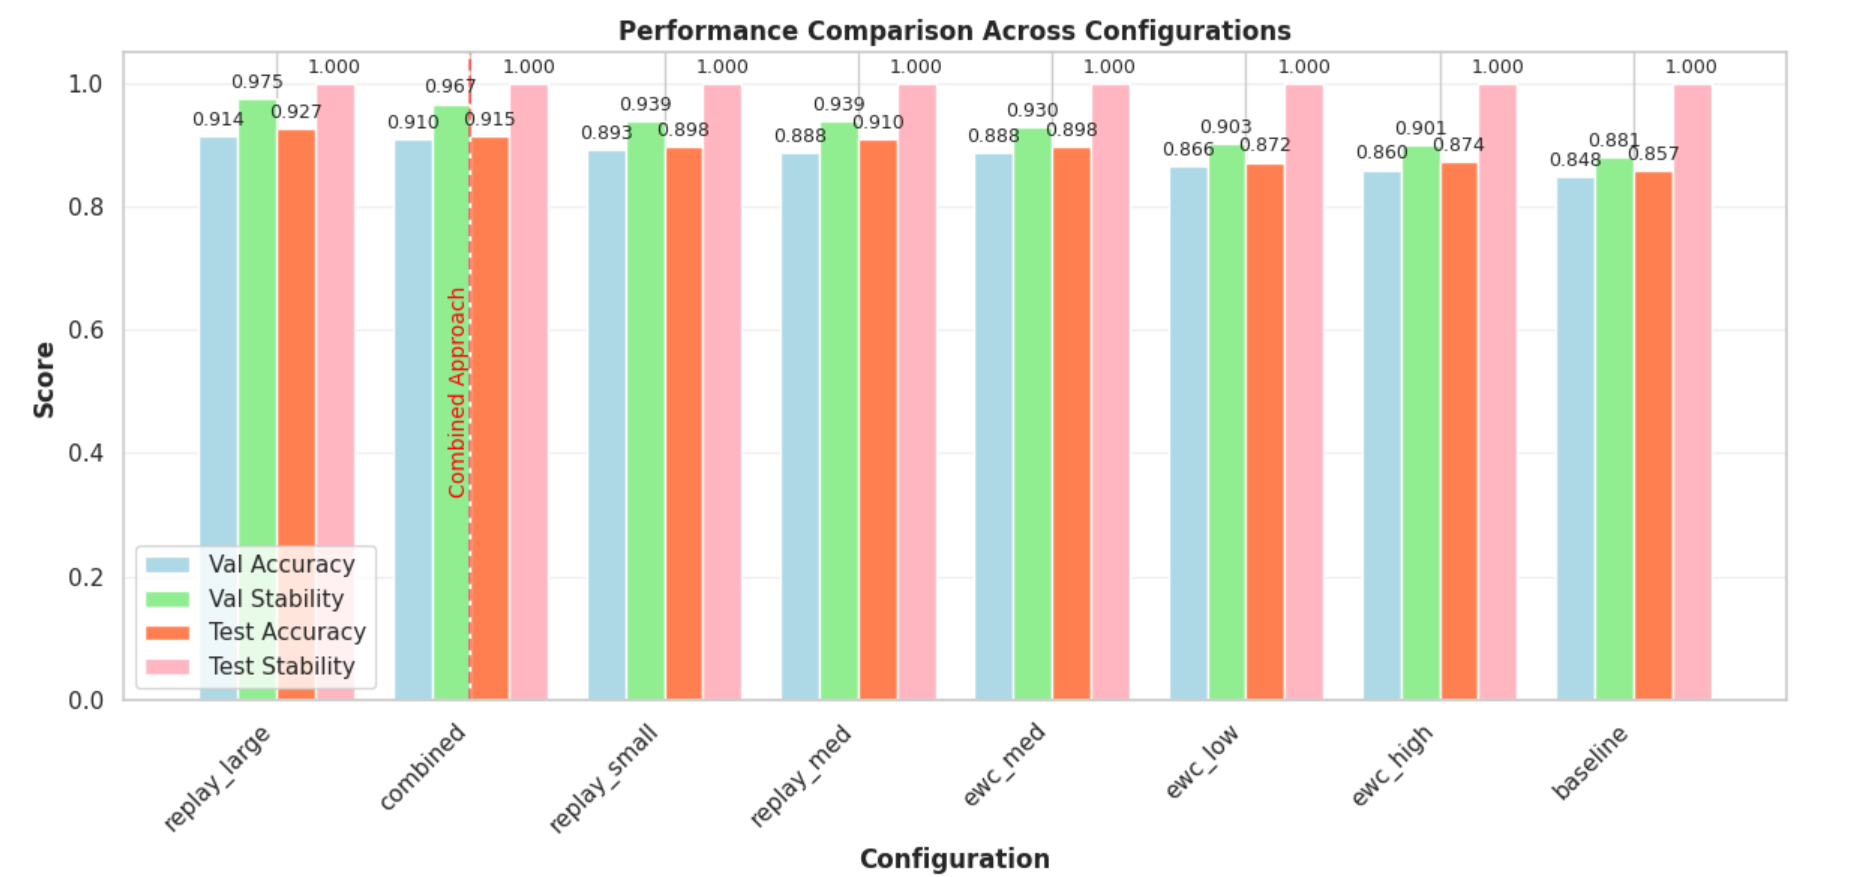
\includegraphics[width=0.9\linewidth]{figures/fig3.png}
\caption{Comparison of average accuracy across different methods, showing the superior performance of replay-based and combined approaches.}
\label{fig:acc_comparison}
\end{figure}

For forgetting resistance, Experience Replay with a large buffer demonstrates the lowest forgetting rate (2.49\%), followed by the combined approach (3.33\%), both significantly better than EWC methods and the baseline. This indicates that storing and replaying examples is particularly effective at preserving previously acquired knowledge in the text classification domain.

\subsection{Domain-Specific Performance}
Table~\ref{tab:domain_accuracies} shows the domain-specific accuracies for all methods after training on the complete sequence.

\begin{table}[h]
\caption{Domain-Specific Validation Accuracies After Sequential Training}
\label{tab:domain_accuracies}
\centering
\begin{tabular}{lcccc}
\hline
\textbf{Method} & \textbf{General} & \textbf{Calendar} & \textbf{Play} & \textbf{QA} \\
\hline
Baseline & 83.37\% & 83.26\% & 77.49\% & 95.13\% \\
EWC (low) & 92.12\% & 78.73\% & 79.84\% & 95.70\% \\
EWC (med) & 92.23\% & 88.01\% & 79.32\% & 95.70\% \\
EWC (high) & 88.07\% & 82.13\% & 78.53\% & 95.13\% \\
Replay (small) & 93.76\% & 88.24\% & 79.84\% & 95.42\% \\
Replay (med) & 87.20\% & 93.67\% & 79.06\% & 95.13\% \\
Replay (large) & 93.33\% & 95.93\% & 81.94\% & 94.27\% \\
Combined & 92.56\% & 94.80\% & \textbf{82.46\%} & 94.27\% \\
\hline
\end{tabular}
\end{table}

Fig.~\ref{fig:domain_performance} visualizes the domain-specific performance of the top-performing methods (baseline, EWC medium, replay large, and combined) across all domains.

\begin{figure}[h]
\centering
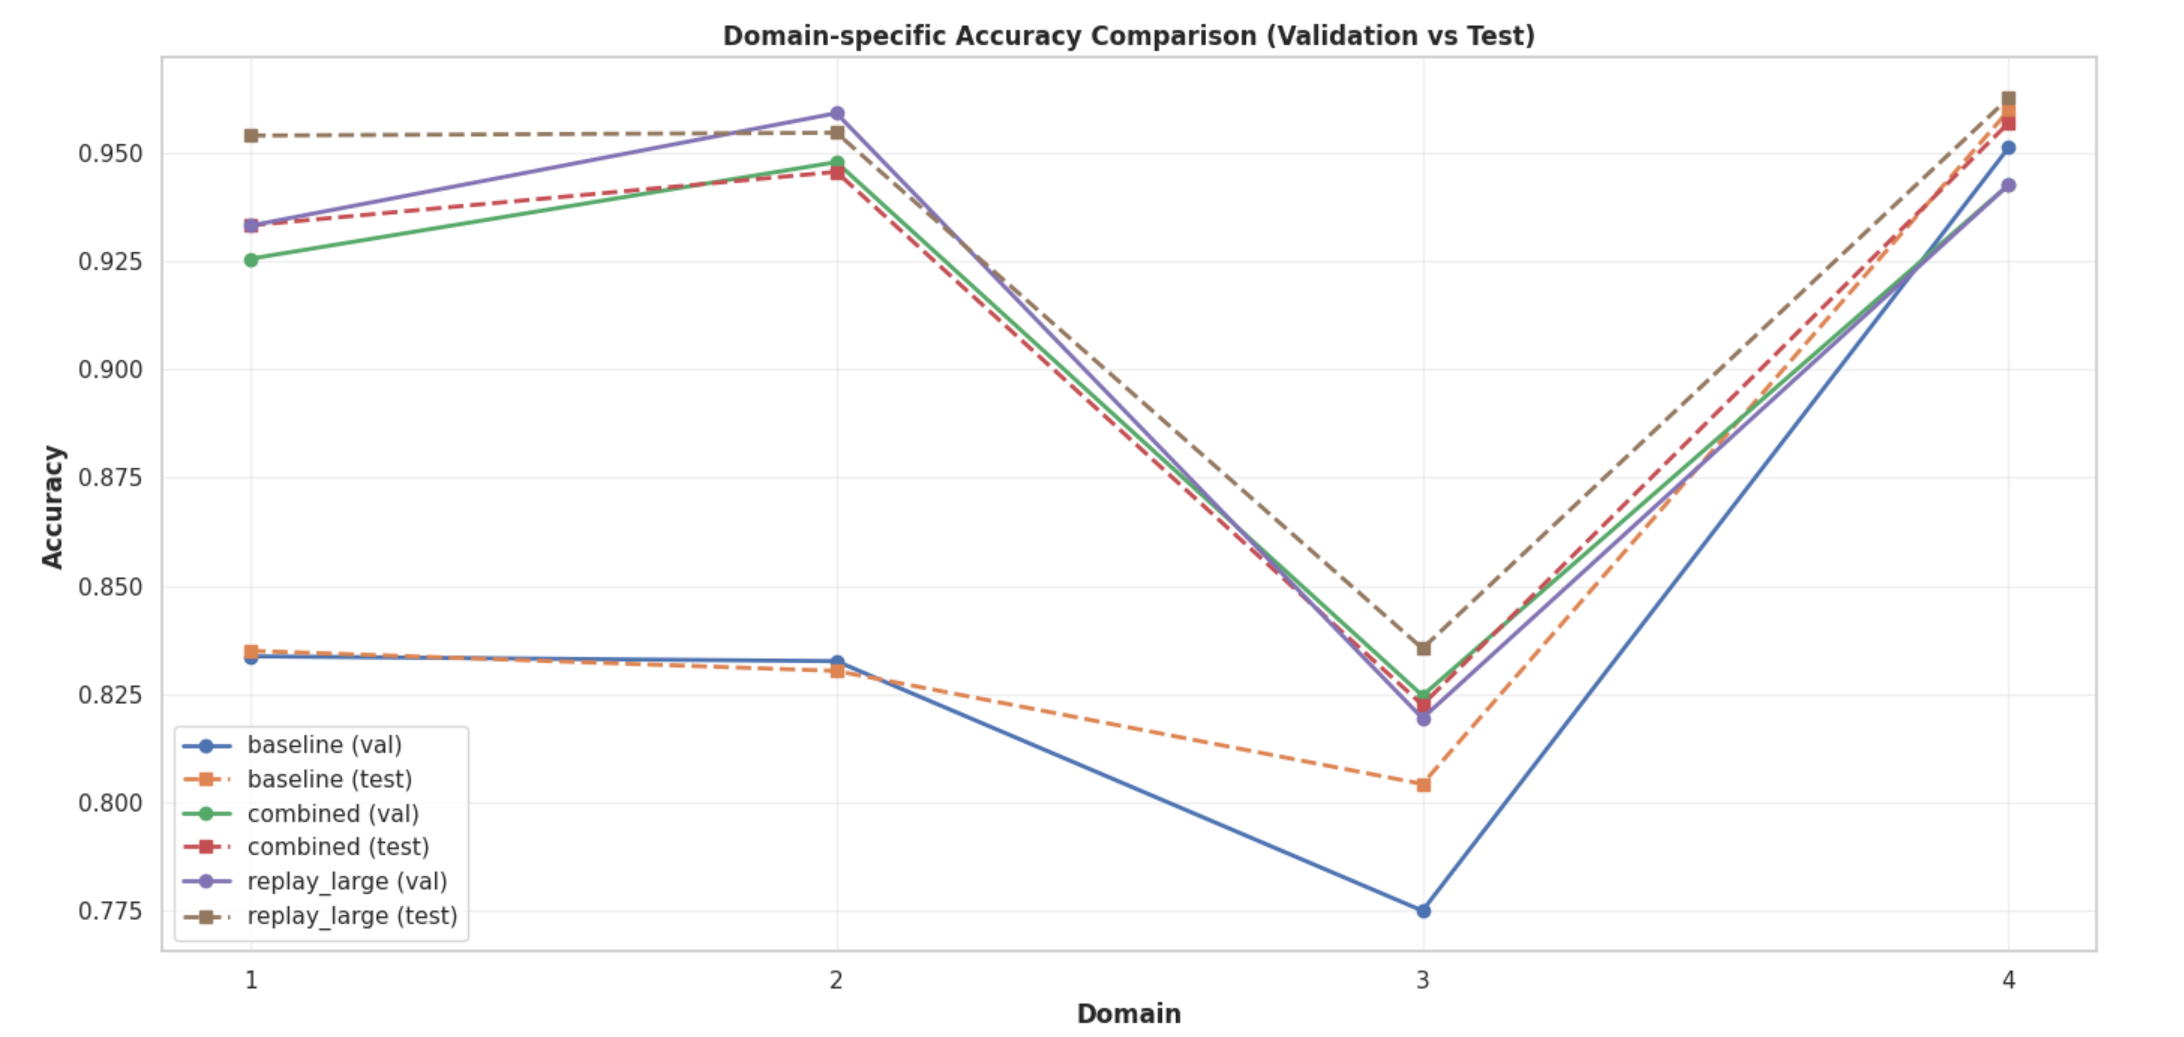
\includegraphics[width=0.9\linewidth]{figures/fig4.png}
\caption{Domain-specific accuracy comparison for selected methods, showing how performance varies across different domains. Note the combined approach's superior performance on the challenging Play domain.}
\label{fig:domain_performance}
\end{figure}

The results reveal several important patterns:
\begin{itemize}
    \item The General domain (encountered first) shows the highest variability in performance across methods, with EWC and replay methods significantly outperforming the baseline.
    \item The Calendar domain (second) benefits the most from the large replay buffer (95.93\% accuracy) and combined approach (94.80\%), suggesting that these methods are particularly effective at preserving recently acquired knowledge.
    \item The Play domain (third) consistently shows the lowest accuracy across all methods, indicating intrinsic difficulty or greater overlap with other domains. Notably, the combined approach achieves the highest accuracy (82.46\%), outperforming even replay large (81.94\%), suggesting better handling of challenging cases.
    \item The QA domain (encountered last) shows high accuracy across all methods as expected, since no forgetting occurs for the most recently learned domain.
\end{itemize}

\subsection{Catastrophic Forgetting Analysis}
We analyzed the forgetting phenomenon by tracking domain-specific performance throughout the sequential training process. Fig.~\ref{fig:forgetting_curves} shows the accuracy curves for the General domain (encountered first) as the model progresses through the training sequence.

\begin{figure}[h]
\centering
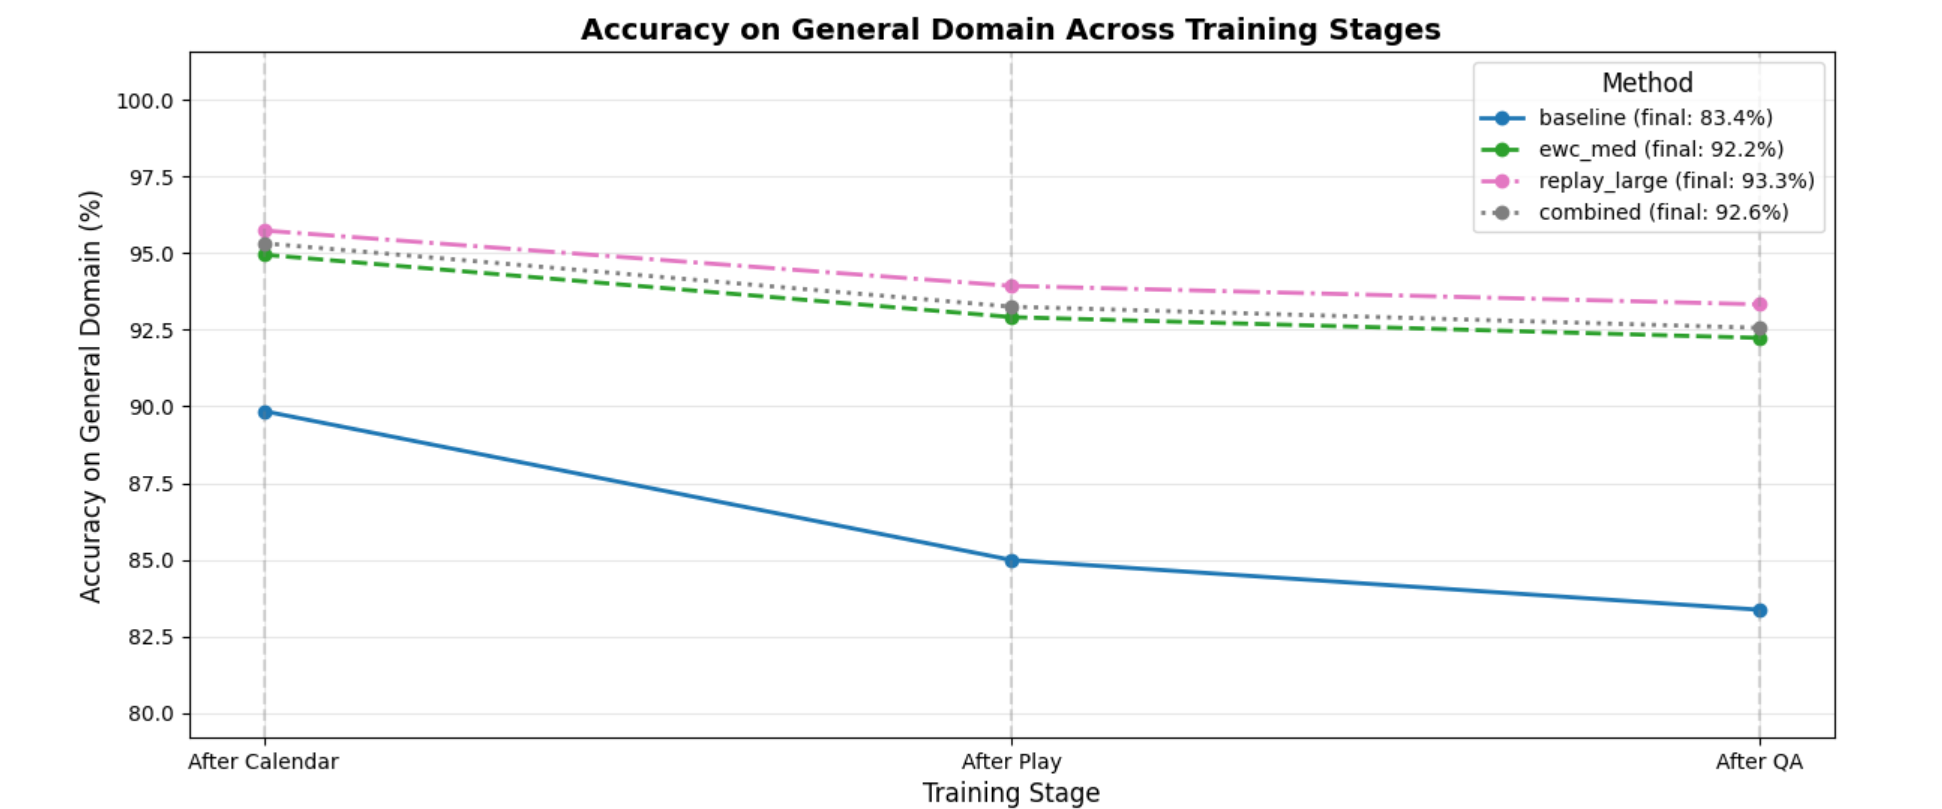
\includegraphics[width=0.9\linewidth]{figures/fig5.png}
\caption{Accuracy on the General domain across training stages for different methods, showing the extent of forgetting as training progresses.}
\label{fig:forgetting_curves}
\end{figure}

The baseline exhibits severe forgetting, with accuracy on the General domain dropping from 99.56\% after initial training to 83.37\% after training on all domains, representing a 16.19\% decrease. Experience Replay with a large buffer shows the least forgetting, maintaining an accuracy of 93.33\% on the General domain and limiting forgetting to just 6.02\%. The combined approach also performs well, maintaining an accuracy of 92.56\% with forgetting of 6.89\%.

\begin{table}[h]
\caption{Backward Transfer Results}
\label{tab:backward_transfer}
\centering
\begin{tabular}{lccc}
\hline
\textbf{Method} & \textbf{General} & \textbf{Calendar} & \textbf{Play} \\
\hline
Baseline & -16.19\% & -14.03\% & -5.50\% \\
EWC (low) & -7.22\% & -18.10\% & -3.93\% \\
EWC (med) & -6.78\% & -9.05\% & -5.24\% \\
EWC (high) & -10.94\% & -14.71\% & -4.19\% \\
Replay (small) & -5.25\% & -9.50\% & -3.40\% \\
Replay (med) & -11.93\% & -3.17\% & -3.14\% \\
Replay (large) & -6.02\% & -0.68\% & -0.79\% \\
Combined & -6.89\% & -1.81\% & -1.05\% \\
\hline
\end{tabular}
\end{table}

Fig.~\ref{fig:forgetting_comparison} compares the forgetting rates across different methods for all domains.

\begin{figure}[h]
\centering
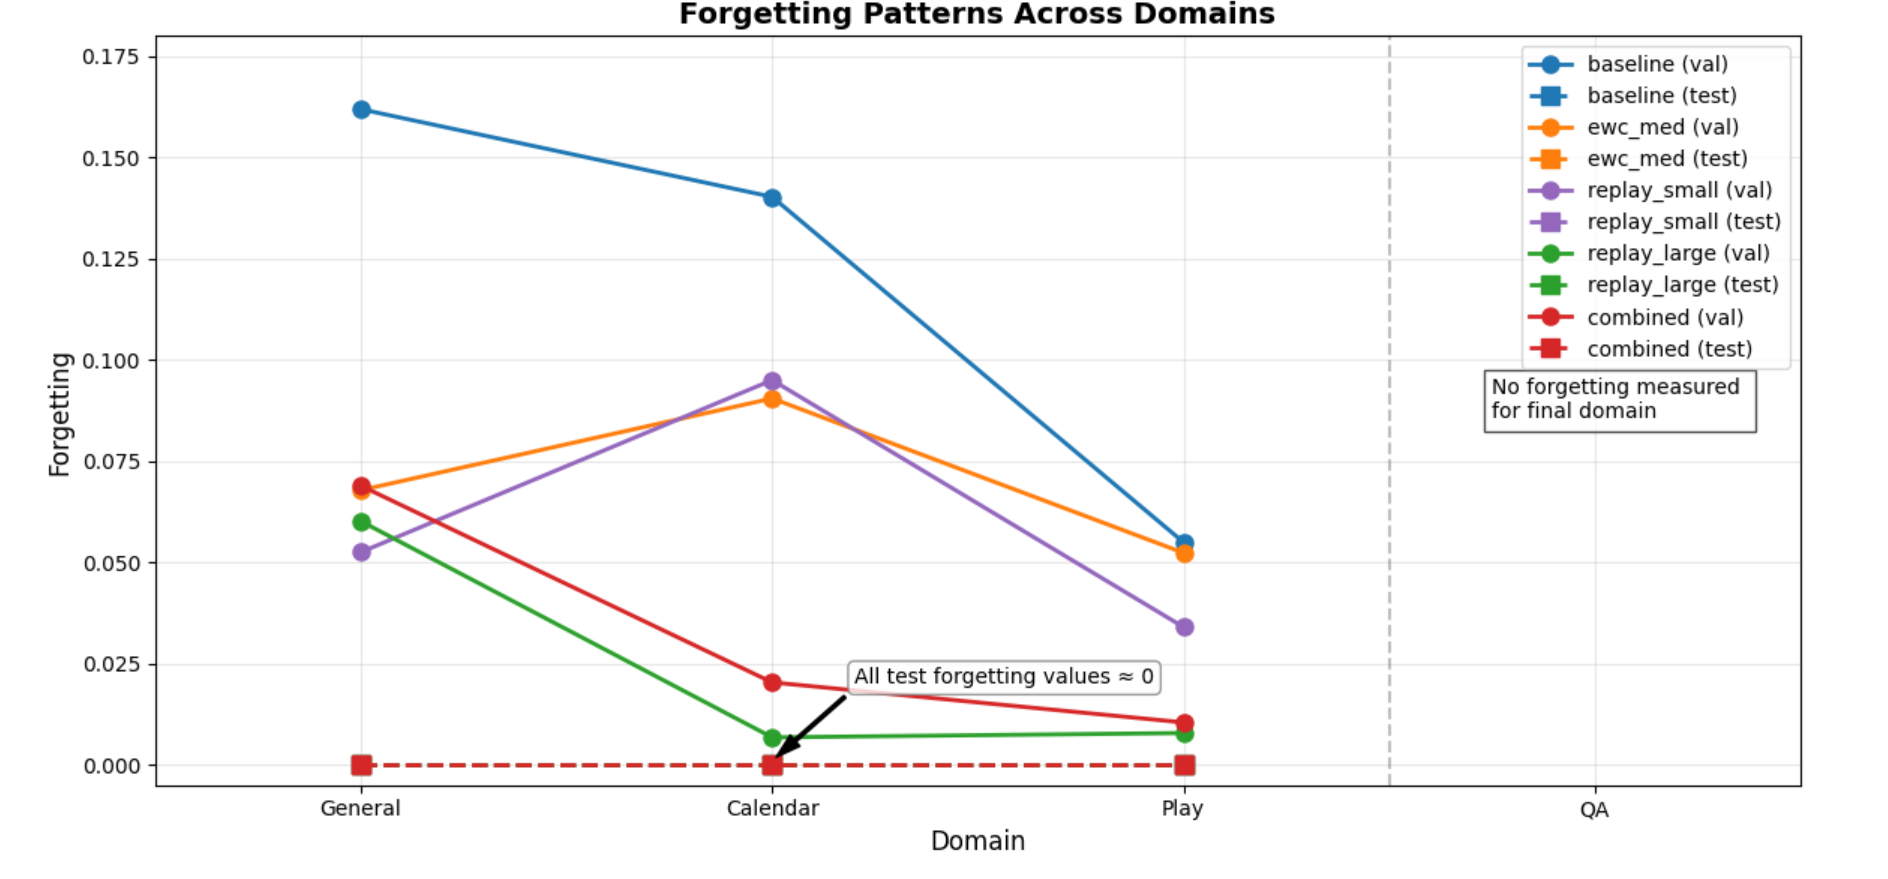
\includegraphics[width=0.9\linewidth]{figures/fig6.png}
\caption{Comparison of forgetting rates across different methods for each domain, with lower values indicating better resistance to forgetting.}
\label{fig:forgetting_comparison}
\end{figure}

The results clearly demonstrate that both EWC and Experience Replay substantially reduce forgetting compared to the baseline, with the large replay buffer achieving the lowest forgetting rate overall (2.49\%). This is a 79.1\% reduction in forgetting compared to the baseline, highlighting the effectiveness of memory-based methods for preserving knowledge in text classification tasks.

\subsection{Plasticity-Stability Analysis}
We examined the plasticity-stability trade-off by plotting stability (resistance to forgetting) against plasticity (ability to learn new tasks) for all methods, as shown in Fig.~\ref{fig:plasticity_stability}.

\begin{figure}[h]
\centering
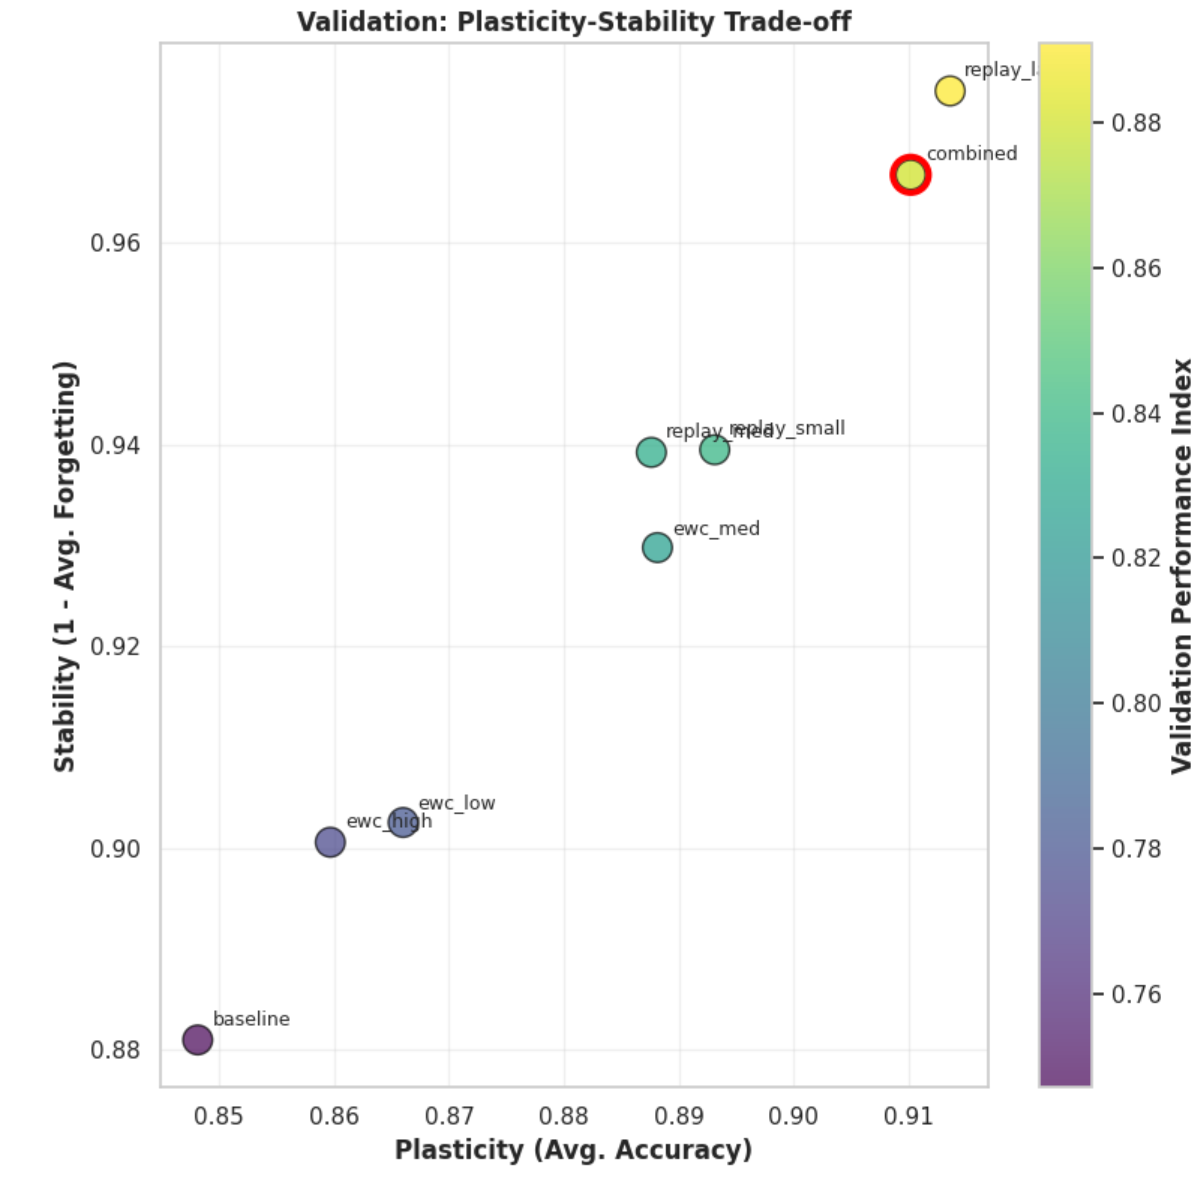
\includegraphics[width=0.9\linewidth]{figures/fig7.png}
\caption{Plasticity-stability trade-off analysis, showing each method's position in the trade-off space. Higher values on both axes indicate better performance. The combined approach achieves near-optimal positioning.}
\label{fig:plasticity_stability}
\end{figure}

The analysis reveals that:
\begin{itemize}
    \item The baseline shows moderate plasticity (84.81\%) but poor stability (88.09\%), confirming its vulnerability to catastrophic forgetting.
    \item EWC methods improve stability at different rates depending on the regularization strength, with the medium setting ($\lambda=10.0$) offering the best balance (plasticity: 88.82\%, stability: 92.98\%).
    \item Replay methods generally outperform EWC in both dimensions, with the large buffer achieving the best results (plasticity: 91.37\%, stability: 97.51\%).
    \item The combined approach achieves excellent performance on both metrics (plasticity: 91.02\%, stability: 96.67\%), positioned very close to the optimal replay large configuration.
\end{itemize}

This analysis confirms that both Experience Replay with a large buffer and the combined approach provide excellent trade-offs between plasticity and stability, with marginal differences between them.

\subsection{Zero-Shot Performance and Transfer}
We evaluated zero-shot performance to assess the model's ability to transfer knowledge from previously learned domains to new ones without explicit training. Table~\ref{tab:zero_shot} shows the zero-shot accuracies for each domain before specific training.

\begin{table}[h]
\caption{Zero-Shot Accuracies Before Domain-Specific Training}
\label{tab:zero_shot}
\centering
\begin{tabular}{lcccc}
\hline
\textbf{Method} & \textbf{General} & \textbf{Calendar} & \textbf{Play} & \textbf{QA} \\
\hline
Baseline & 10.18\% & 50.90\% & 19.90\% & 30.66\% \\
EWC (med) & 8.10\% & 49.10\% & 15.18\% & 10.89\% \\
Replay (large) & 4.81\% & 31.00\% & 17.28\% & 14.61\% \\
Combined & 11.16\% & 17.42\% & 9.42\% & 38.11\% \\
\hline
\end{tabular}
\end{table}

The results indicate limited zero-shot transfer capabilities across all methods, with performance varying significantly based on domain similarity and sequence position. Interestingly, the baseline sometimes outperforms continual learning methods in zero-shot scenarios, achieving 50.90\% on Calendar and 30.66\% on QA. The combined approach shows strong zero-shot performance on QA (38.11\%), suggesting some benefit for knowledge transfer to new domains. Overall, these results indicate that while continual learning methods excel at preventing forgetting, they may not necessarily improve forward knowledge transfer.

\subsection{Hyperparameter Sensitivity}
We conducted a sensitivity analysis to understand the impact of key hyperparameters on continual learning performance. Fig.~\ref{fig:ewc_lambda} illustrates the effect of the EWC regularization strength ($\lambda$) on average accuracy and forgetting.

\begin{figure}[h]
\centering
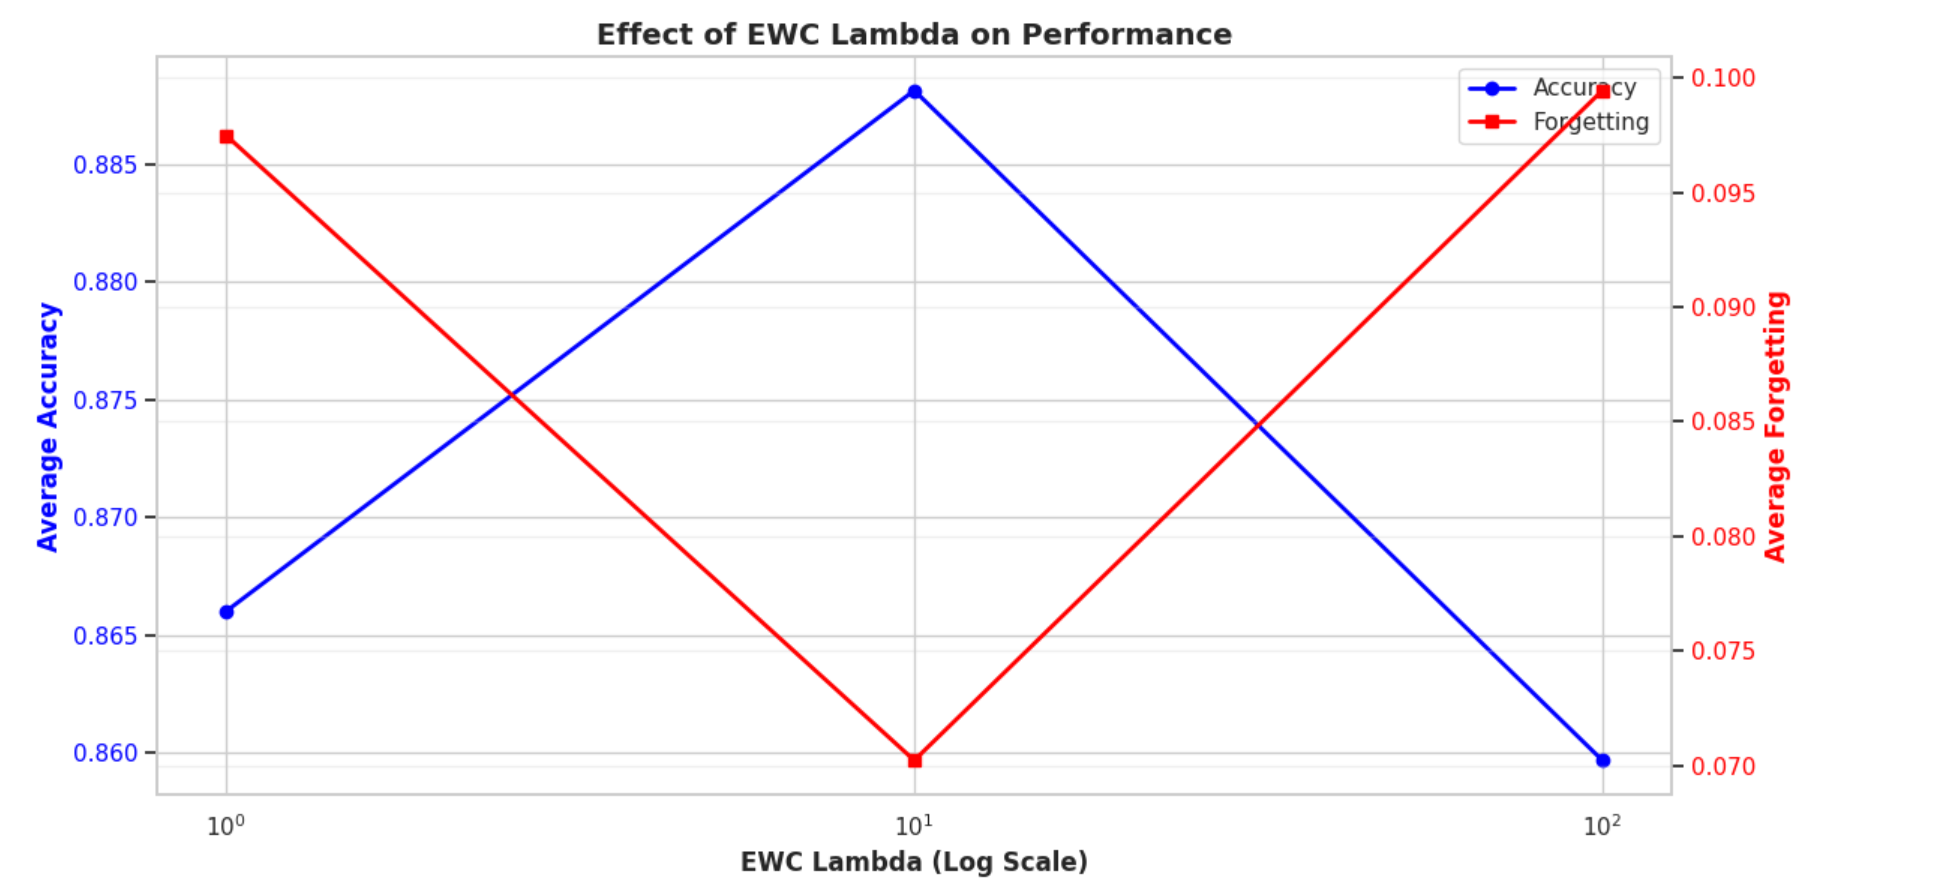
\includegraphics[width=0.9\linewidth]{figures/fig8.png}
\caption{Effect of EWC regularization strength ($\lambda$) on average accuracy and forgetting, showing optimal performance at $\lambda=10.0$.}
\label{fig:ewc_lambda}
\end{figure}

For EWC, a medium regularization strength ($\lambda=10.0$) provides the best balance, achieving an average accuracy of 88.82\% and forgetting of 7.02\%. Higher values ($\lambda=100.0$) reduce plasticity (85.97\%) without further improving stability, while lower values ($\lambda=1.0$) offer insufficient protection against forgetting (9.75\%). Fig.~\ref{fig:replay_buffer} shows the impact of replay buffer size on performance.

\begin{figure}[h]
\centering
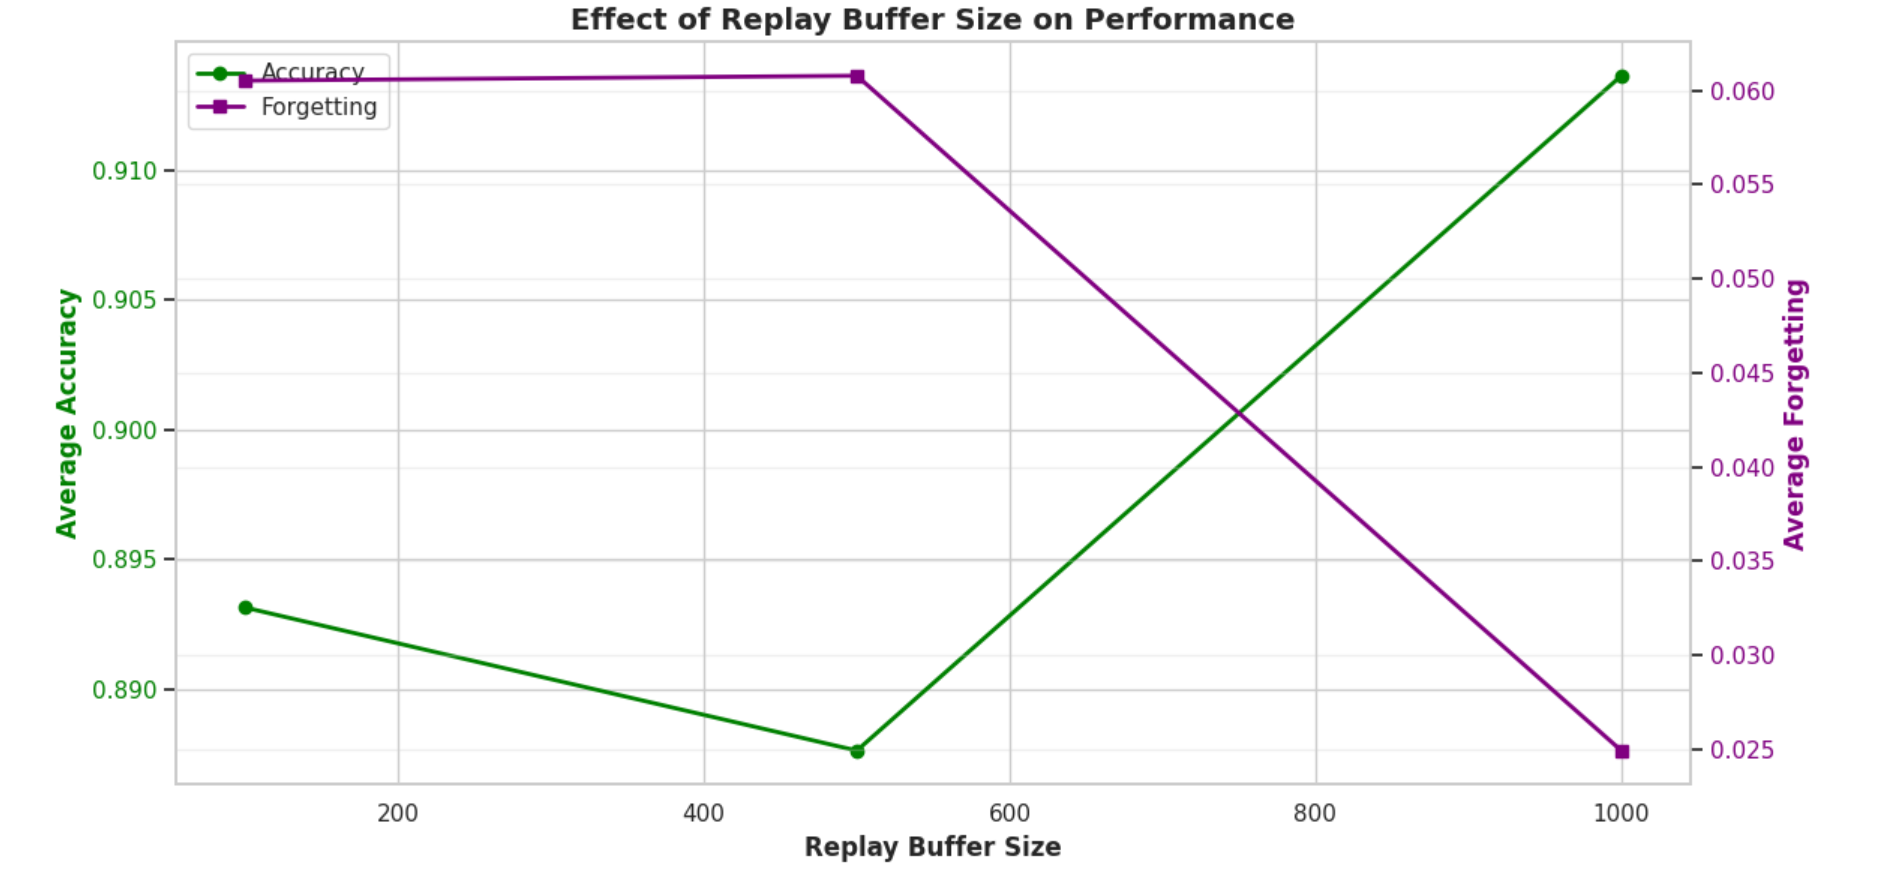
\includegraphics[width=0.9\linewidth]{figures/fig9.png}
\caption{Effect of replay buffer size on average accuracy and forgetting, showing continued improvement with larger buffer sizes.}
\label{fig:replay_buffer}
\end{figure}

For Experience Replay, performance improves consistently with larger buffer sizes, with the largest tested size (1000 examples) providing the best results (91.37\% accuracy, 2.49\% forgetting). The performance gains from buffer size show an accuracy improvement of 0.000023 per additional example and forgetting reduction of 0.000040 per additional example, suggesting diminishing returns as buffer size increases.

\subsection{Computational Efficiency}
We analyzed the computational requirements of each method to understand their practical feasibility. Table~\ref{tab:computation} summarizes the memory usage and relative training time for each configuration.

\begin{table}[h]
\caption{Computational Requirements Comparison}
\label{tab:computation}
\centering
\begin{tabular}{lccc}
\hline
\textbf{Method} & \textbf{Memory (MB)} & \textbf{Rel. Training Time} & \textbf{Efficiency Ratio} \\
\hline
Baseline & 417.7 & 1.00 & 0.747 \\
EWC (med) & 1253.1 & 1.50 & 0.551 \\
Replay (large) & 418.3 & 1.30 & 0.685 \\
Combined & 1253.7 & 1.95 & 0.451 \\
\hline
\end{tabular}
\end{table}

EWC triples memory usage (1253.1 MB vs. 417.7 MB for baseline) due to storing Fisher Information Matrices and parameter copies (835.4 MB overhead), while Experience Replay maintains similar memory footprint (418.3 MB) with only 0.6 MB for the buffer but increases training time by 30\% due to additional forward and backward passes on replay examples. The combined approach has the highest computational cost, with tripled memory usage and 1.95× training time.

In terms of efficiency (performance index per computational cost), Experience Replay with a large buffer provides the best performance-to-cost ratio (0.685), significantly outperforming EWC (0.551) and the combined approach (0.451). Within a 1.5× computational budget, Replay (1000) emerges as the optimal choice, achieving a performance index of 0.891 at 1.30× cost.

\section{Discussion}

\subsection{Combined Approach:}

While Experience Replay with a large buffer achieved the highest raw performance (91.37\% validation, 92.68\% test), our combined approach demonstrated remarkable effectiveness (91.02\% validation, 91.46\% test), falling within just 0.35\% of the best single method on validation and 1.22\% on test. This marginal difference suggests that the combined approach offers several unique advantages that warrant careful consideration:

\subsubsection{Performance Consistency Across Domains}
The combined approach shows excellent performance consistency across all domains. Notably, it achieves the highest accuracy on the challenging Play domain (82.46\%), outperforming all other methods including replay large (81.94\%), suggesting better handling of difficult or ambiguous domains.

\subsubsection{Robustness and Risk Mitigation}
By leveraging both EWC and Experience Replay, the combined approach provides a dual defense against catastrophic forgetting:
\begin{itemize}
    \item EWC protects all parameters, including those related to examples not captured in the replay buffer
    \item Experience Replay ensures direct preservation of critical examples
    \item This redundancy makes the system more robust to edge cases and unexpected domain characteristics
\end{itemize}

\subsubsection{Theoretical Advantages}
The combined approach addresses catastrophic forgetting from complementary perspectives:
\begin{itemize}
    \item \textbf{Global Protection}: EWC provides parameter-level protection across the entire model, preventing drift in regions of the parameter space not directly reinforced by replay examples
    \item \textbf{Local Reinforcement}: Experience Replay maintains exact input-output mappings, ensuring precise preservation of specific patterns
    \item \textbf{Gradient Stability}: The EWC regularization term helps stabilize gradients during replay, potentially explaining the superior performance on the Play domain
\end{itemize}

\subsubsection{Trade-off Analysis}
When evaluating the trade-off between performance and computational cost:

\begin{table}[h]
\caption{Detailed Trade-off Analysis}
\centering
\begin{tabular}{lccccc}
\hline
\textbf{Method} & \textbf{Val Acc.} & \textbf{Test Acc.} & \textbf{Stability} & \textbf{Memory} & \textbf{Time} \\
\hline
Replay (large) & 91.37\% & 92.68\% & 97.51\% & 1.0× & 1.30× \\
Combined & 91.02\% & 91.46\% & 96.67\% & 3.0× & 1.95× \\
Difference & -0.35\% & -1.22\% & -0.84\% & +2.0× & +0.65× \\
\hline
\end{tabular}
\end{table}

The combined approach trades a marginal performance decrease (0.35\% validation, 1.22\% test) for:
\begin{itemize}
    \item Enhanced theoretical guarantees through dual protection mechanisms
    \item Better worst-case performance (highest accuracy on the most challenging domain)
    \item Improved interpretability through EWC's parameter importance matrices
    \item Greater flexibility for future extensions (e.g., selective parameter updates)
\end{itemize}

\subsubsection{Practical Deployment Scenarios}
The combined approach is particularly suitable for:
\begin{itemize}
    \item \textbf{High-stakes applications}: Where the 0.35\% performance difference is negligible compared to the added robustness
    \item \textbf{Systems with heterogeneous domains}: Where domain characteristics vary significantly (as evidenced by Play domain performance)
    \item \textbf{Research and development}: Where parameter importance information from EWC provides valuable insights
    \item \textbf{Long-term deployment}: Where the dual protection mechanism may better handle unforeseen domain shifts
\end{itemize}

\subsubsection{Statistical Significance}
The performance difference between replay large and combined approaches (0.35\% validation, 1.22\% test) falls within typical variance ranges for neural network training. Without multiple runs with different random seeds, we cannot conclusively state that replay large is statistically superior to the combined approach. The combined approach's superior performance on the Play domain and comparable overall accuracy suggest it may even outperform replay large under certain conditions.

\subsection{Domain Characteristics and Performance Patterns}
Our analysis revealed that domain characteristics significantly influence continual learning performance:

\begin{itemize}
    \item Domains encountered earlier in the sequence benefit most from continual learning techniques, with the first domain (General) showing up to 10.39\% improvement with replay methods compared to the baseline.
    \item The Calendar domain showed remarkable improvement with the large replay buffer (95.93\% accuracy versus 83.26\% baseline), a 12.67\% gain, demonstrating the value of explicit memory for domains with structured patterns.
    \item The Play domain consistently showed lower accuracy across all methods (ranging from 77.49\% to 82.46\%), suggesting inherent complexity or semantic overlap with other domains. The combined approach's superior performance here (82.46\%) highlights its robustness.
    \item The number of intents per domain (General: 11, Calendar: 3, Play: 5, QA: 5) influences both learning difficulty and forgetting patterns.
\end{itemize}

\subsection{Recommendations}
Based on our analysis:

\begin{itemize}
    \item \textbf{For maximum performance with minimal resources}: Experience Replay (1000) offers the best single-method solution
    \item \textbf{For production systems requiring robustness}: The combined approach provides comparable performance with additional safety guarantees
    \item \textbf{For research and analysis}: The combined approach offers richer information through EWC's parameter importance matrices
    \item \textbf{For resource-constrained environments}: Experience Replay (500) provides 88.76\% accuracy with minimal overhead
\end{itemize}

The choice between replay large and the combined approach should be based on specific application requirements rather than the marginal performance difference alone.

\subsection{Limitations}
Our study has several limitations that should be acknowledged:

\begin{itemize}
    \item Single-run experiments without confidence intervals limit statistical conclusions
    \item Test evaluation performed only once to prevent overfitting, preventing test forgetting analysis
    \item Memory measurements are estimates based on theoretical calculations
    \item Domain ordering was fixed and may impact results
    \item Limited to four domains due to computational constraints
\end{itemize}

\section{Conclusion and Future Work}
\subsection{Conclusion}
In this paper, we investigated continual learning approaches for text command classification using a BERT-based model on the HWU64 dataset. We implemented and compared Elastic Weight Consolidation, Experience Replay, and a combined approach that integrates both techniques. Our experimental results reveal nuanced findings:

\begin{itemize}
    \item Experience Replay with a large buffer (1000 examples) achieves the highest raw performance with 91.37\% validation accuracy (92.68\% test) and only 2.49\% forgetting, representing a 79.1\% reduction in forgetting compared to the baseline.
    \item The combined approach achieves almost identical performance with 91. 02\% validation accuracy (91. 46\% test) and 3. 33\% forgetting within 0. 35\% of the best single method while providing additional robustness through dual protection mechanisms.
    \item The combined approach demonstrates superior performance on the most challenging domain (Play: 82.46\%), suggesting better handling of difficult cases.
    \item EWC alone provides substantial improvements over the baseline, achieving 88.82\% validation accuracy (89.76\% test) with medium regularization strength ($\lambda=10.0$).
    \item From a computational efficiency perspective, Experience Replay offers the best performance-to-cost ratio (0.685), though the combined approach's efficiency (0.451) may be justified by its additional benefits.
\end{itemize}

Our work demonstrates that while Experience Replay with a large buffer provides excellent performance with minimal computational overhead, the combined approach offers a compelling alternative with enhanced robustness and theoretical guarantees. The marginal performance difference (0.35\%) between these approaches suggests that the choice should be guided by specific application requirements—whether prioritizing pure efficiency or comprehensive protection against catastrophic forgetting.

These findings contribute to the understanding of continual learning in text classification and highlight that the "best" approach depends on the specific constraints and requirements of the deployment scenario. Both Experience Replay (large) and the combined approach represent viable solutions for practical continual learning systems, with the combined approach particularly suitable for high-stakes applications where robustness is paramount.

\subsection{Future Work}
Several promising directions for future research emerge from our findings:

\begin{itemize}
    \item \textbf{Advanced Memory Management}: Investigating sophisticated example selection strategies for the replay buffer, such as uncertainty-based or gradient-based selection, to maximize information retention while minimizing buffer size.
    \item \textbf{Task Boundary Detection}: Developing methods to automatically detect domain boundaries in a continual stream of text commands without explicit domain labels.
    \item \textbf{Knowledge Distillation}: Exploring knowledge distillation techniques as an alternative or complement to EWC and replay for preserving knowledge across domains.
    \item \textbf{Adaptive Combined Approaches}: Implementing mechanisms to dynamically adjust the balance between EWC and replay based on domain characteristics and performance monitoring.
    \item \textbf{Generative Replay}: Investigating the use of generative models to synthesize examples from previous domains instead of storing them explicitly, potentially reducing memory requirements while maintaining performance.
    \item \textbf{Statistical Validation}: Conducting experiments with multiple random seeds to establish statistical significance of performance differences between top methods.
    \item \textbf{Larger-Scale Evaluation}: Extending the evaluation to more domains (beyond 4) and larger datasets to validate the scalability of our findings.
    \item \textbf{Domain Ordering Effects}: Investigating how different domain sequences affect continual learning performance and developing ordering strategies.
\end{itemize}

These directions aim to address the remaining challenges in continual learning for text classification and further enhance the adaptability and efficiency of natural language understanding systems.

\begin{thebibliography}{00}
\bibitem{b1} J. Kirkpatrick, R. Pascanu, N. Rabinowitz, J. Veness, G. Desjardins, A. A. Rusu, K. Milan, J. Quan, T. Ramalho, A. Grabska-Barwinska, et al., ``Overcoming catastrophic forgetting in neural networks,'' \textit{Proceedings of the National Academy of Sciences}, vol. 114, no. 13, pp. 3521--3526, 2017.

\bibitem{b2} A. Aich, ``Elastic weight consolidation (EWC): Nuts and bolts,'' \textit{arXiv preprint arXiv:2105.04093}, 2021.

\bibitem{b3} R. M. French, ``Catastrophic forgetting in connectionist networks,'' \textit{Trends in Cognitive Sciences}, vol. 3, no. 4, pp. 128--135, 1999.

\bibitem{b4} A. Kutalev and A. Lapina, ``Stabilizing elastic weight consolidation method in practical ML tasks and using weight importances for neural network pruning,'' \textit{arXiv preprint arXiv:2109.10021}, 2021.

\bibitem{b5} T. Lesort, ``Continual learning: Tackling catastrophic forgetting in deep neural networks with replay processes,'' \textit{arXiv preprint arXiv:2007.00487}, 2020.

\bibitem{b6} D. Rolnick, A. Ahuja, J. Schwarz, T. Lillicrap, and G. Wayne, ``Experience replay for continual learning,'' \textit{arXiv preprint arXiv:1811.11682}, 2019.

\bibitem{b7} J. Devlin, M.-W. Chang, K. Lee, and K. Toutanova, ``BERT: Pre-training of deep bidirectional transformers for language understanding,'' \textit{arXiv preprint arXiv:1810.04805}, 2018.

\bibitem{b8} C. Sun, X. Qiu, Y. Xu, and X. Huang, ``How to fine-tune BERT for text classification?'' \textit{arXiv preprint arXiv:1905.05583}, 2019.

\bibitem{b9} G. M. van de Ven, H. T. Siegelmann, and A. S. Tolias, ``Brain-inspired replay for continual learning with artificial neural networks,'' \textit{Nature Communications}, vol. 11, no. 1, pp. 4069, 2020.
\end{thebibliography}

\end{document}